\documentclass[a4paper,12pt]{article}
\usepackage{mathrsfs}
\usepackage[utf8]{inputenc}
\usepackage[spanish]{babel}
\usepackage{amsmath}
\usepackage{amsfonts}
\usepackage{amssymb} 
\usepackage{graphicx} 
\usepackage{hyperref} 
\usepackage{wrapfig}
\usepackage{enumitem}
\usepackage{fancyhdr}
\usepackage{float}
\usepackage{eurosym}
\usepackage{color}
\usepackage{circuitikz}
\usepackage{titling}
\usepackage{hyperref}
\usepackage{media9}
\usepackage{lipsum}
\usepackage{tocbibind}
\usepackage{listings}
\usepackage{tabularx}
\usepackage{tcolorbox}
\usepackage{bookmark}
\usepackage{media9}
\usepackage[table]{xcolor}
\definecolor{lightblue}{RGB}{228, 244, 253}
\usepackage{listings}
\usepackage{color}

\definecolor{dkgreen}{rgb}{0,0.6,0}
\definecolor{gray}{rgb}{0.5,0.5,0.5}
\definecolor{mauve}{rgb}{0.58,0,0.82}

\lstset{frame=tb,
  language=Python,
  inputencoding=utf8,
  extendedchars=true,
  aboveskip=3mm,
  belowskip=3mm,
  showstringspaces=false,
  columns=flexible,
  basicstyle={\small\ttfamily},
  numbers=none,
  numberstyle=\tiny\color{gray},
  keywordstyle=\color{blue},
  commentstyle=\color{dkgreen},
  stringstyle=\color{mauve},
  breaklines=true,
  breakatwhitespace=true,
  tabsize=3,
  literate=%
    {á}{{\'a}}1
    {é}{{\'e}}1
    {í}{{\'i}}1
    {ó}{{\'o}}1
    {ú}{{\'u}}1
    {ñ}{{\~n}}1
    {č}{{\v{c}}}1
}
\usepackage[left=3cm,right=3cm,top=3cm,bottom=4cm]{geometry}
\sloppy

\pagestyle{fancy}
\providecommand{\abs}[1]{\lvert#1\rvert}
\providecommand{\norm}[1]{\lVert#1\rVert}

%%% Para las cabeceras
\newcommand{\hsp}{\hspace{20pt}}
\newcommand{\HRule}{\rule{\linewidth}{0.5mm}}
\headheight=50pt
%%% 
\newcommand{\vacio}{\textcolor{white}{ .}}

%%% Para que las ecuaciones se numeren
%%% con el número de sección y el de ecuación.
\renewcommand{\theequation}{\thesection.\arabic{equation}}


% Color azul para algunos 
% textos de la portada
\definecolor{azulportada}{rgb}{0.16, 0.32, 0.75}

%%%% Azul para textos de headings
\definecolor{azulinterior}{rgb}{0.0, 0.2, 0.6}

%%%%%%%%%%%%%%%%%%%%%%%%%%%%%%%%
%%%%%% Datos del proyecto %%%%%%
%%%%%%%%%%%%%%%%%%%%%%%%%%%%%%%%
%%%TÍTULO
%%% Escribirlo en minúsculas, el programa
%%% lo pondrá en mayúsculas en la portada.

\title{Procesamiento de imágenes}

%%%% AUTORES
\author{Lydia Ruiz Martínez \and Pablo Tuñón Laguna}

%%%%%%%%%%%%%%%%%%%%%
%%%%%%%%%%%%%%%%%%%%
\begin{document}

%%%%%%%%%%%%%%%%%%%%%%%%%%%%%%%
%%%%%%%%%%%%%%%%%%%%%%%%%%%%%%%
\begin{titlepage} %%%%% Aquí no hay que tocar nada.
	%%%% Las siguientes instrucciones generarán automáticamente
	%%%% la portada de tu proyecto.
	%%% Cambio de la estructura de esta página
\newgeometry{left=0.6cm,top=1.3cm,bottom=1.2cm}

\fbox{\parbox[c]{18.5cm}{
\begin{center}
\vspace{1.5cm}
{\fontfamily{ptm}\fontsize{24}{28.8}\selectfont{Universidad Pontificia de Comillas}}\\
[3.5em]
{\fontfamily{ptm}\fontsize{24}{5}\selectfont{ICAI}}\\
[4.5em]
{\fontfamily{ptm}\fontsize{28}{5}\selectfont{LABORATORIO 2}}\\
[2cm]
{\fontfamily{ptm}\fontsize{24}{5}\selectfont{Visión por Ordenador I}}\\
[2cm]

% Autor del trabajo de investigación
\textcolor{azulportada}{\fontfamily{ptm}\fontsize{16}{5}\selectfont{\theauthor}}\\
[2cm]
% Título del trabajo
\textcolor{azulportada}
{\fontfamily{ptm}\fontsize{30}{5}\selectfont{\textsc{\thetitle}}}\\
%{\Huge\textbf{\thetitle}}\\
[1.2cm]

\includegraphics[width=10cm]{fonts/Logo ICAI.png}
\\[1.8cm]

{\fontfamily{ptm}\fontsize{16}{5}\selectfont{Curso 2024-2025}}\\
[4cm]
\end{center}
}}
\end{titlepage}
 
 \restoregeometry
 %%%% Volvemos a la estructura de la página normal

%%%%%%%%%%%%%%%%%%%%%%%%%%%%%%

{%\Large

%%%Encabezamiento y pie de página
%%% También se genera automáticamente
%%% Mejor no tocarlo mucho.
\renewcommand{\headrulewidth}{0.5pt}
\fancyhead[R]{
\textcolor{azulportada}{\fontfamily{ptm}\fontsize{10}{3}\selectfont{Laboratorio 2 de Visión por Ordenador I}}\\
{\fontfamily{ptm}\fontsize{10}{3}\selectfont{\theauthor}}}
\fancyhead[L]{
  \textcolor{azulinterior}{\fontfamily{ptm}\fontsize{14}{4}\selectfont{\textbf{\thetitle}}}\\
}

\pagestyle{fancy}
\renewcommand{\footrulewidth}{0.5pt}
\fancyfoot[L]{\footnotesize Universidad Pontificia de Comillas (ICAI) --- curso 2024-2025}
\fancyfoot[C]{\vacio}
\fancyfoot[R]{\footnotesize Página \thepage}

%%%%%%%%%%%%%%%%%%%%
\newpage

\renewcommand{\contentsname}{Índice}
\addtocontents{toc}{\protect\setcounter{tocdepth}{-1}} % Quita el índice de la tabla de contenidos
\tableofcontents
\addtocontents{toc}{\protect\setcounter{tocdepth}{2}}

\newpage


\section{Introducción}


\vspace{1cm}

El procesamiento de imágenes es un área fundamental de la visión por ordenador, esta se enfoca en la manipulación y el análisis
de imágenes digitales. A diferencia de un ser humano, que puede interpretar imágenes de manera intuitiva, un ordenador necesita
algoritmos específicos que le permitan extraer información útil de las matrices de píxeles que componen cada imagen. Estos 
algoritmos permiten a los sistemas de visión por ordenador realizar tareas como la segmentación, la detección de bordes 
y la aplicación de filtros, convirtiendo datos visuales en información comprensible.

\vspace{0.5cm}

La segmentación de imágenes por color es una técnica crucial que permite identificar y aislar objetos de interés en una imagen 
basándose en sus características cromáticas. Este proceso es esencial en múltiples aplicaciones, desde la automatización 
industrial hasta la medicina, donde la identificación precisa de regiones de interés puede marcar la diferencia en el análisis
y la toma de decisiones. La capacidad de un ordenador para diferenciar colores y reconocer patrones en el espacio de color 
adecuado es un paso inicial vital en la interpretación de las imágenes.

\vspace{0.5cm}

La aplicación de filtros es otra herramienta relevante en el procesamiento de imágenes. El operador gaussiano, con combinación con los filtros de
Sobel o el de Canny se utilizan para suavizar imágenes, eliminar el ruido y detectar bordes, respectivamente. La detección de bordes
es especialmente relevante, ya que resalta las transiciones significativas en una imagen, facilitando la identificación de 
 formas y estructuras. Al aplicar y comparar estos filtros, se puede evaluar tanto la variación en la calidad de la imagen como
la eficiencia en la detección de bordes.

\vspace{0.5cm}

Finalmente, el uso de operadores morfológicos complementa estas técnicas al permitir la manipulación de la estructura de componentes
de una imagen píxel a píxel. Se trata de un enfoque fundamental para mejorar los resultados de la segmentación y la 
detección que además permite desarrollar una comprensión más profunda de las características presentes en las imágenes. En el siguiente estudio, 
se llevarán a cabo implementaciones de las técnicas mencionadas a través de las librerías de Python OpenCv, Imageio y Numpy con el objetivo de
desarrollar un conocimiento práctico de las herramientas de procesamiento de imágenes y su aplicación en la visión por ordenador.

\newpage


\section{Segmentación}


\vspace{1cm}

La segmentación de imágenes por colores es una técnica sencilla y útil en aplicaciones en las que se tiene un gran control
sobre las condiciones de contorno: iluminación, tipo de objeto que se espera encontrar, color de fondo, etc.
En un primer momento se realizaron pruebas de segmentación de imágenes con los colores naranja y blanco, sin embargo, posteriormente
se realizó una adaptación que permite al usuario segmentar cualquier color de su elección.

\vspace{0.5cm}

\subsection{Carga de imágenes}

\vspace{0.5cm}

Todo proceso de visión por ordenador comienza con la carga de las imágenes a procesar, sin embargo hay múltiples formas de llevar 
a cabo este proceso. En el caso de la segmentación de imágenes por color este paso es especialmente importante. Para cargar las imágenes
a partir de su ruta de almacenamiento (obtenida a través de \textit{glob.glob()}) se pueden usar dos procesos análogos:

\vspace{0.5cm}

\begin{itemize}
  \item \textit{cv2.imread()}: La función de la librería \textit{cv2} carga las imágenes en formato RGB.

  \item \textit{imageio.imread()}: La función de la librería \textit{imageio} carga las imágenes en formato BGR.
\end{itemize}

\vspace{0.5cm}

Esta transformación de formato es relevante ya que si se diseña un algoritmo de segmentación de colores en un espacio, no funcionará 
si recibe otro espacio de color ya que los canales de color se interpretan de manera diferente. Esto se puede observar al cargar 
la misma imagen sin realizar ninguna transformación y visualizarla en ambos formatos:

\vspace{0.5cm}

\begin{figure}[H]
  \centering
  \begin{minipage}[t]{0.35\textwidth}
      \centering
      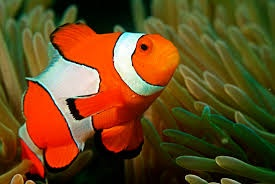
\includegraphics[width=\textwidth]{processed_data/cv2_charged_0.jpg} 
      \caption{Imagen 1 cargada con \textit{cv2.imread()}, formato RGB, autoría propia.}
      \label{fig:cv2_charged}
  \end{minipage}
  \hfill
  \begin{minipage}[t]{0.35\textwidth}
      \centering
      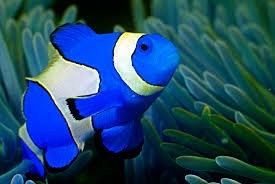
\includegraphics[width=\textwidth]{processed_data/imageio_charged_0.jpg}
      \caption{Imagen 1 cargada con \textit{imageio.imread()}, formato RGB, autoría propia.}
      \label{fig:imageio_charged}
  \end{minipage}
\end{figure}

\subsection{Segmentación monocolor}

\vspace{0.5cm}

Cargadas ya las imágenes se procede a transformarlas al espacio de color HSV ya que genera un mayor contraste : Hue (brillo), Saturation (saturación) y Value (valor).
Para ello se usa la función \textit{cv2.cvtColor()} de OpenCV, que recibe como argumentos la imagen y el espacio de color al que se desea transformar. Una vez que las 
imágenes estén en el espacio de color adecuado, se procede a generar máscaras necesarias, que permiten segmentar los colores de interés. A continuación se muestran los
valores de los umbrales HSV para las imágenes de naranja y blanco:

\vspace{0.5cm}

{\centering
$\text{Naranja}_{min}$; H: 1, S: 190, V: 200 \\
$\text{Naranja}_{max}$; H: 255, S: 255, V: 255 \\
$\text{Blanco}_{min}$; H: 0, S: 0, V: 150 \\
$\text{Blanco}_{max}$; H: 255, S: 50, V: 255\\}

\vspace{0.5cm}

Posteriormente se hace uso de la función \textit{cv2.inRange()} de OpenCV, que recibe como argumentos la imagen en el espacio de color HSV, los valores mínimos y máximos 
aceptados para cada canal de color. Esta función devuelve una máscara binaria en la que los píxeles que cumplen con los umbrales establecidos se marcan como blancos y 
los que no, permanecen negros. Finalmente, se emplea la función \textit{cv2.bitwise\_and()}, que opera examinando bit a bit y realizando la operación AND. Esta función se aplica 
sobre la máscara blanca creada y sobre la imagen original, de tal manera que sólo se seleccionen aquellos bits marcados como unos en la máscara, tengan el color que tengan 
en la imagen original. Cabe destacar que se segmenta cualquier color que esté en la zona ''asociada al color a segmentar'' porque en la figura 4 se puede observar una tonalidad 
del naranja cercana al amarillo o en la figura 6 como hay fragmentos del segmento que no son de color blanco puro. Esto se debe al hecho de que los filtros diseñados no son perfectos,
se han diseñado para que seleccionen la máxima cantidad de color de un conjunto genérico de imágenes, eliminar ese ''ruido'' sobre los segmentos de determinadas imágenes puede 
producir ''overfitting'' lo cual reduce las posibilidades de generalización de la segmentación.

\vspace{0.5cm}

\begin{figure}[H]
  \centering
  \begin{minipage}[t]{0.3\textwidth}
      \centering
      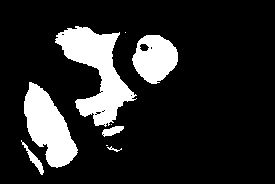
\includegraphics[width=\textwidth]{processed_data/orange_mask_0.jpg} 
      \caption{Máscara naranja de la imagen 1, autoría propia.}
      \label{fig:white_mask}
  \end{minipage}
  \hfill
  \begin{minipage}[t]{0.3\textwidth}
      \centering
      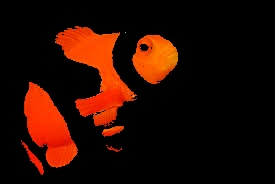
\includegraphics[width=\textwidth]{processed_data/orange_segmented_0.jpg}
      \caption{Segmentación naranja de la imagen 1, autoría propia.}
      \label{fig:white_segmented}
  \end{minipage}
  
\end{figure}

\begin{figure}[H]

  \begin{minipage}[t]{0.3\textwidth}
      \centering
      
\includegraphics[width=\textwidth]{processed_data/white_mask_0.jpg}
      \caption{Máscara blanco de la imagen 1, autoría propia.}
      \label{fig:orange_mask}
  \end{minipage}
  \hfill
  \begin{minipage}[t]{0.3\textwidth}
      \centering
      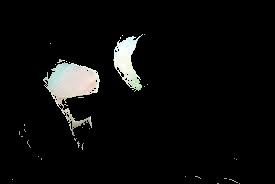
\includegraphics[width=\textwidth]{processed_data/white_segmented_0.jpg}
      \caption{Segmentación blanco de la imagen 1, autoría propia.}
      \label{fig:orange_segmented}
  \end{minipage}
\end{figure}

\subsection{Segmentación multicolor}

\vspace{0.5cm}

El segmentado de múltiples colores se entiende como la creación de una máscara binaria por cada color de interés realizando posteriormente una superposición en 
una más genérica. Dado que las máscaras son binarias, basta con hacer una operación OR entre ellas para obtener la máscara que con la que filtrar las imágenes originales. 
Para ejemplificar este proceso, se han segmentado los colores naranja, blanco de la imagen 1, así como el blanco, rojo, verde, azul, amarillo y gris del logo de 
''Redbull King of the Air'' (el verde es el color por defecto del fondo de un png):

\vspace{0.5cm}

\begin{figure}[H]
  \centering
  \begin{minipage}[t]{0.3\textwidth}
      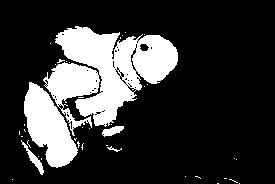
\includegraphics[width=\textwidth]{processed_data/fish_mask_0.jpg} 
      \caption{Máscara multicolor de la imagen 1, autoría propia.}
      \label{fig:multicolor_mask}
  \end{minipage}
  \hfill
  \begin{minipage}[t]{0.3\textwidth}
      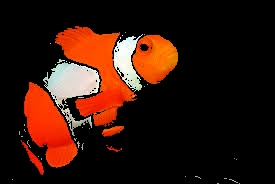
\includegraphics[width=\textwidth]{processed_data/fish_segmented_0.jpg}
      \caption{Segmentación multicolor de la imagen 1, autoría propia.}
      \label{fig:multicolor_segmented}
  \end{minipage}

\end{figure}

\begin{figure}[H]
  
  \begin{minipage}[t]{0.6\textwidth}
    
\includegraphics[width=0.3\textwidth]{data/king_of_the_air.png}
    \caption{Logo de ''Redbull King of the Air'',\\https://www.redbull.com/es-es/events/king-of-the-air.}
    \label{fig:redbull_original}
  \end{minipage}
  \hfill
  \hspace{1.5cm}
  \begin{minipage}[t]{0.6\textwidth}
    \includegraphics[width=0.3\textwidth]{processed_data/king_of_the_air_segmented.jpg}
    \caption{Segmentación multicolor\\del logo de''Redbull King of the Air'',\\ autoría propia.}
    \label{fig:redbull_segmentation}
  \end{minipage}

\end{figure}


\section{Operador Gaussiano y detectores de bordes: Sobel y Canny}


\vspace{1cm}

El filtrado de imágenes es una técnica fundamental en el procesamiento de imágenes que permite mejorar la calidad de las imágenes, eliminar el ruido y resaltar 
características de interés. Habitualmente el filtrado se emplea para resaltar o extraer los bordes de una umagen, ya que estos contienen información relevante
sobre la forma y estructura de los elementos presentes en la imagen. Se recuerda que un ordenador cuando procesa una imagen no puede interpretarla de forma intuitiva,
por lo que una imagen de un cubo, aunque el ojo humano pueda identificarlo, para un ordenador es simplemente un conjunto de píxeles, de esta manera se puede extraer un
conjunto de bordes, que si se unen de forma adecuada, se puede identificar el cubo.  Para el filtrado de imágenes se ha estudiado el operador gaussiano así como los 
filtros Sobel y Canny.

\vspace{0.5cm}

\subsection{Operador Gaussiano}

\vspace{0.5cm}

El operador gaussiano pertenece al conjunto de los operadores LSI, este tipo de operadores cumplen con la propiedad de linealidad y desplazamiento invariante. La propiedad de
linealidad implica que los píxeles de salida son una combinación lineal pesada de los píxeles de entrada (es decir una convolución), mientras que la propiedad de desplazamiento invariante 
implica que se realiza la misma operación en todos los píxeles de la imagen. El operador gaussiano se emplea para suavizar las imágenes, eliminando el ruido y reduciendo la 
cantidad de detalles presentes, esto se consigue tomando los pesos de la combinación de píxeles de un kernel (o matriz cuadrada de número impar de columnas) gaussiano. 
La función gaussiana se define como:

\vspace{0.5cm}

\begin{equation}
  G(i, j) = \frac{1}{2\pi\sigma^2}e^{-\frac{i^2 + j^2}{2\sigma^2}}
\end{equation}

\vspace{0.5cm}

A través de la ecuación anterior se extrae el kernel gaussiano, este se aplica a la imagen original mediante la función \textit{cv2.filter2D()}. Dicha función recombina los 
píxeles de la imagen original con los pesos del kernel, reduciendo el detalle pero proporcionando una mayor difernciación de los elementos de la imagen. Precisamente por dicha 
característica se aplicará el operador antes de aplicar otros más especificos4. A continuación se muestra la aplicación del filtro gaussiano a la imagen 1: 

\vspace{0.5cm}

\begin{figure}[H]

\begin{minipage}[t]{0.4\textwidth}
    \centering
    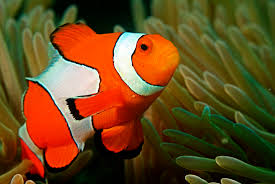
\includegraphics[width=\textwidth]{data/000.jpg} 
    \caption{Imagen 1, set de imagenes proporcionadas.}
    \label{fig:original-image}
\end{minipage}
\hfill
\hspace{1.5cm}
\begin{minipage}[t]{0.4\textwidth}
    \centering
    \includegraphics[width=\textwidth]{processed_data/gaussian_blur_0.jpg} 
    \caption{Operador gaussiano sobre la imagen 1, autoría propia.}
    \label{fig:gaussian_filter}
\end{minipage}

\end{figure}

\subsection{Detector Sobel}

\vspace{0.5cm}

El operador Sobel es uno de los empleados en la detección de bordes. Este operador se basa en la convolución de la imagen original nuevamente con kernels de pesado.
En el entorno del estudio realizado, se usa el kernel de Sobel respecto a los ejes x e y, que se definen como:

\vspace{0.5cm}

\[
  S_x = \begin{bmatrix} -1 & -2 & -1 \\ 0 & 0 & 0 \\ 1 & 2 & 1 \end{bmatrix} \quad S_y =  \begin{bmatrix} -1 & 0 & 1 \\ -2 & 0 & 2 \\ -1 & 0 & 1 \end{bmatrix}
\]

\vspace{0.5cm}

El operador actua como una versión discreta del gradiente de una imagen, el cual se define como el vector que apunta en la dirección de la mayor variación de intensidad.
La aplicación del operador Sobel a una imagen permite resaltar los bordes de la imagen, ya que los píxeles de los bordes presentan una mayor variación de intensidad
en comparación con los píxeles interiores. El operador se rota para no tener en cuenta los píxeles de alta variación en la dirección del borde a resaltar. A continuación se 
muestra una imagen con la detección sobel calculada a través de distintas formas:

\vspace{0.5cm}

\begin{figure}[H]

  \begin{minipage}[t]{0.4\textwidth}
      \centering
      \includegraphics[width=\textwidth]{processed_data/sobel_0.jpg} 
      \caption{Aplicación de sobel con opencv sobre la imagen 1, autoría propia.}
      \label{fig:cv2-sobel}
  \end{minipage}
  \hfill
  \hspace{1.5cm}
  \begin{minipage}[t]{0.4\textwidth}
      \centering
      \includegraphics[width=\textwidth]{processed_data/scikit_sobel_0.jpg} 
      \caption{Aplicación de sobel con scikit sobre la imagen 1, autoría propia.}
      \label{fig:scikit-sobel}
  \end{minipage}
  
\end{figure}

\vspace{0.5cm}

La figura 13 muestra el resultado de aplicar el operador sobel(en vertical y horizontal) a través de la función \textit{cv2.filter2D()}
mientras que la figura 14 representa el resultado de aplicar el operador sobel a través de la función \textit{skimage.filters.sobel()} de la librería scikit-image.
Ambas funciones son equivalentes, esto se puede observar en la gran similitud entre las imágenes filtradas, aunque la función de scikit-image, parece que marcad
de forma más suave los bordes de la imagen.

\vspace{0.5cm}

\subsubsection{Filtro de Prewitt}

El filtro de Prewitt es un operador de detección de bordes aparentemente idéntico al de Sobel, con una pequeña variación en el kernel. Se sustituyen
los doses por unos de tal manera que se pesa de la misma forma los píxeles de la imagen en la dirección del borde:

\vspace{0.5cm}

\[
  P_x = \begin{bmatrix} -1 & -1 & -1 \\ 0 & 0 & 0 \\ 1 & 1 & 1 \end{bmatrix} \quad P_y =  \begin{bmatrix} -1 & 0 & 1 \\ -1 & 0 & 1 \\ -1 & 0 & 1 \end{bmatrix}
\]

\vspace{0.5cm}

La aplicación del filtro de Prewitt sobre la imagen 1 se muestra en las figura 15 y 16, en ella se puede apreciar la gran similitud con las imágenes 13 y 14. 
Esto se debe a la similitud entre los kernels de Sobel y Prewitt, que aunque no son idénticos, son muy parecidos:

\vspace{0.5cm}

\begin{figure}[H]

  \begin{minipage}[t]{0.35\textwidth}
      \centering
      \includegraphics[width=\textwidth]{processed_data/prewitt_0.jpg} 
      \caption{Aplicación de prewitt con opencv sobre la imagen 1, autoría propia.}
      \label{fig:cv2-prewitt}
  \end{minipage}
  \hfill
  \hspace{1.5cm}
  \begin{minipage}[t]{0.35\textwidth}
      \centering
      \includegraphics[width=\textwidth]{processed_data/scikit_prewitt_0.jpg} 
      \caption{Aplicación de prewitt con scikit sobre la imagen 1, autoría propia.}
      \label{fig:scikit-prewitt}
  \end{minipage}
  
\end{figure}

\vspace{0.5cm}

\subsection{Detector de bordes Canny}

\vspace{0.5cm}

El operador Canny toma el fundamento teórico de los operadores anteriores, pero añade un paso adicional de ''supresión de
no máximos'', dicho procesado es un algoritmo de reducción de ruido alrededor de los bordes detectados con Sobel o Prewitt.
Esta limpieza se realiza clasificando un pixel en las variaciones más comunes de borde (0º, 45º, 90º y 135º) para posteriormente
comparar el valor del pixel con los de los píxeles vecinos en la dirección del borde. En caso de que el pixel sea el máximo del 
conjunto evaluado, se mantiene, en caso contrario se elimina. De esta manera sólo se conservan los píxeles más relevantes de 
los bordes detectados, eliminando el posible ruido así como las detecciones menos precisas. A continuación se la aplicación de
un filtro Canny a la imagen 1:

\vspace{0.5cm}

\begin{figure}[H]
  \centering
  \begin{minipage}[t]{0.35\textwidth}
      \centering
      \includegraphics[width=\textwidth]{processed_data/canny_0.jpg} 
      \caption{Aplicación de Canny con opencv sobre la imagen 1, autoría propia.}
      \label{fig:cv2-canny}
  \end{minipage}
  \hfill
  \begin{minipage}[t]{0.35\textwidth}
      \centering
      \includegraphics[width=\textwidth]{processed_data/scikit_canny_0.jpg} 
      \caption{Aplicación de Canny con scikit sobre la imagen 1, autoría propia.}
      \label{fig:scikit-canny}
  \end{minipage}
\end{figure}

\vspace{1cm}

La figura 17 muestra el resultado de aplicar el operador Canny (en vertical y horizontal) a través de la función \textit{cv2.filter2D()}, 
para luego suprimir el ruido a mediante la función \textit{utils.non\_max\_suppression()}. La imagen 18 representa el resultado de aplicar 
el operador Canny con la función \textit{skimage.feature.canny()} de la librería scikit-image. De todos los casos estudiados, este es el 
único en el que se aprecia una diferencia significativa entre las librerías de filtrado usadas. Es cierto que la imagen 17 no contiene nada 
de ruido, pero apenas es capaz de identificar los bordes del pez, mientras que la imagen 18 es capaz de identificar los bordes del pez, 
pero también los del fondo. Es más, parece que no produce una mejora significativa ya que al comparar la imagen 18 con la 16 se ve como algunos 
bordes del pez en lugar de ser más finos y precisos son más imprecisos y dobles. Con el objetivo de ampliar la supresión de ruido y mejorar 
la detección de bordes se valora la opción de modificar la función de \textit(utils.non\_max\_suppression()) para que sea algo menos restrictiva.
También se considera que realizar erosión (un proceso que se explicará más adelante) sobre la imagen filtrada con sobel o prewitt puede mejorar
la futura supresión de ruido.

\vspace{0.5cm}

\subsection{Mejora de detección de bordes}

\vspace{0.5cm}

Tal y como se comentó en el apartado del operador gaussiano, aplicarlo antes de aplicar cualquier otro borde es una buena práctica ya que 
permitirá un mejor filtrado de los bordes. Es una práctica que se ha llevado a cabo en todas las ejecuciones de los operadores de detección de bordes,
pero que no se explicó en su momento debido a que no se tenía el fundamento teórico sobre el funcionamiento de los operadores. Con el fin de no volver a
realizar todos los filtrados de bordes para llegar a un análisis similar al ya producido, se va a hacer la siguiente prueba. Se va a aplicar un ruido
gausiano sobre las imágenes originales, esto implica que a cada píxel se le sumará un valor aleatorio de acuerdo a una distribución normal de media 127 
y desviación típica 25. La media es el valor medio que puede tomar un píxel y la desviación típica es una que permite ver el ruido en la imagen sin tardar
un tiempo excesivo en ejecutar:

\vspace{0.5cm}

\begin{figure}[H]
  \centering
  \begin{minipage}[t]{0.3\textwidth}
      \centering
      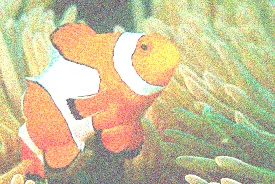
\includegraphics[width=\textwidth]{noisy_data/noisy_0.jpg} 
      \caption{Ruido gaussiano sobre la imagen 1, autoría propia.}
      \label{fig:gaussian_noise}
  \end{minipage}
\end{figure}

\vspace{0.5cm}

A continuación se va a aplicar el operador Sobel sobre la imagen con ruido de dos formas, en la primera no se va a aplicar el operador gaussiano mientras 
que en la segunda se va a realizar el filtrado gaussiano antes de aplicar el operador Sobel:

\vspace{0.5cm}

\begin{figure}[H]
  \centering  
  \begin{minipage}[t]{0.4\textwidth}
    \centering
    \includegraphics[width=\textwidth]{processed_data/noisy_sobel_0.jpg}
    \caption{Aplicación de Sobel sobre la imagen 1 con ruido, autoría propia.}
    \label{fig:noisy-sobel}
  \end{minipage}
  \hspace{1.5cm}
  \centering
  \begin{minipage}[t]{0.4\textwidth}
    \centering
    \includegraphics[width=\textwidth]{processed_data/noisy_sobel_gauss_0.jpg}
    \caption{Aplicación de Gauss y posteriormente de Sobel sobre la imagen 1 con ruido, autoría propia.}
    \label{fig:noisy-gaussian-sobel}
  \end{minipage}
\end{figure}

\vspace{0.5cm}

Tal y como se puede observar en las figuras anteriores, la aplicación del operador gaussiano antes de extraer los bordes con Sobel permite una mejor detección de los mismos.
No sólo se eliminan los puntos detectados debido al ruido, sino que se resaltan más los bordes del pez. Este resultado es el esperado ya que el operador gaussiano se encarga de
suavizar la imagen, eliminando el ruido y resaltando las características de interés. Es por ello por lo que se ha realizado un filtrado gaussiano antes de aplicar los operadores
expuestos hasta el momento.

\newpage

\section{Operadores morfológicos}

A lo largo de la siguiente sección, se estudiarán los operadores morfológicos de dilatación y de erosión. Los operadores morfológicos son relevantes ya que permiten manipular una imágen 
píxel a píxel. Las aplicaciones son múltiples y variadas en el campo de la visión por ordenador: segmentación, detección de bordes... Un operador morfológico se basa en asignar a un píxel 
el máximo o el mínimo de los valores de los píxeles vecinos. Es cierto que se podría aplicar un operador morfológico a una imagen en color, pero habría que dividir la imagen en canales y 
únicamente sería una repetición del proceso. También se puede aplicar sobre una escala de grises, pero para obtener imágenes más puras desde un principio se van a usar imágenes binarias.

\vspace{0.5cm}

\subsection{Binarización de una imagen}

\vspace{0.5cm}

La binarización de una imagen es un proceso en el que se convierte una imagen en escala de grises a una imagen cuyos únicos colores presentes son el blanco y el negro. Esto se realiza a través
de un threshold o límite, una vez establecido, todo pixel con un valor inferior al mismo será asociado al 0 (negros) mientras que el resto de píxeles se igualarán a 1 (blancos).

\vspace{0.5cm}

\subsection{Dilatación}

\vspace{0.5cm}

La dilatación toma el valor máximo de un conjunto de píxeles, cabe destacar que el conjunto de píxeles a evaluar es una cuadrícula de 3x3 donde la casilla central es el píxel cuyo valor se 
considera variar en función de los píxeles vecinos. Para llevar a cabo este proceso en una imagen y no dejar los píxeles del borde sin evaluar, se ha realizado primero un padding sobre la imagen.
Con este objetvo se ha aplicado la función \textit{np.pad()} a la que se le ha indicado que debe añadir una línea de píxeles negros alrededor de la imagen principal de tal manera que al evaluar 
una zona en búsqueda de máximos este borde no afecte. Finalmente se puede aplicar el operador, esto permite una ampliación de las partes blancas de la imagen binaria, haciendo más gruesas esas líneas
y por tanto reduciendo la precisión de los detalles:

\vspace{0.5cm}

\begin{figure}[H]
  \centering
  \begin{minipage}[t]{0.4\textwidth}
    \centering
    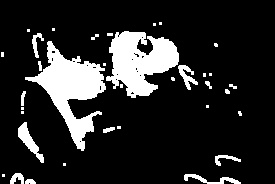
\includegraphics[width=\textwidth]{processed_data/dilated_0.jpg}
    \caption{Dilatación de la binarización de la imagen 1, autoría propia.}
    \label{fig:dilated}

  \end{minipage}
\end{figure}

\vspace{0.5cm}

\subsection{Erosión}

\vspace{0.5cm}

La erosión es un procesado casi idéntico a la dilatación con la única modificación que en lugar de tomar los máximos de un conjunto de píxeles vecinos, se toman los mínimos de los píxeles.
Es por ello que para que el padding no afecte a la asignación de valores, en este caso el borde extra será de píxeles blancos. Al realizar la erosión se logra una reducción en las partes blancas
de la imagen, haciendo más finas las líneas y por tanto aumentando la precisión de la imagen pero no de los detalles finos:

\vspace{0.5cm}

\begin{figure}[H]
  \centering
  \begin{minipage}[t]{0.4\textwidth}
    \centering
    
\includegraphics[width=\textwidth]{processed_data/eroded_0.jpg}
    \caption{Erosión de la binarización de la imagen 1, autoría propia.}
    \label{fig:eroded}

  \end{minipage}
\end{figure}

\end{document}



